% all-in-one cheatsheet layout (Michael Franzen, 2013)
\documentclass[a4paper]{article}

% geometry settings
\usepackage[top=2cm, bottom=2.5cm, left=2cm, right=2cm]{geometry}

% font settings
%\usepackage[light,math]{kurier}
\usepackage[T1]{fontenc}
\usepackage[utf8]{inputenc}
\usepackage{marvosym}
\usepackage{amssymb}
\usepackage{amsfonts}
\usepackage{amsmath}
\usepackage{amsthm}

% colors
\usepackage{xcolor}
\definecolor{lightgray}{gray}{0.8}

% formatting
\usepackage{paralist}
\usepackage{multicol}
\usepackage{tabularx}
\usepackage{Tabbing}
\usepackage{booktabs}
\usepackage{fancyhdr}
\usepackage{url}
\usepackage[framemethod=tikz]{mdframed}
\pagestyle{fancy}

% math
\usepackage{array}
\usepackage{eqnarray}
\usepackage{mathtools}

% figures
\usepackage{wrapfig}
\usepackage{subfig}

% figure modules
\usepackage{graphicx}
\usepackage{tikz}
\usetikzlibrary{positioning,calc, shapes}
\usepackage{algorithm2e}
\usepackage{verbatim}	

% TOC & Glossary
\usepackage{sectsty}
\usepackage[nottoc,notlof,notlot]{tocbibind}
\usepackage[titles,subfigure]{tocloft}

% commands
\usepackage{xargs}
\usepackage{ifthen}

% head line
\fancyhf{}
\chead{Graph Theory - Sheet 2 - \today\\J. Batzill (1698622), M. Franzen (1696933), J. Labeit (1656460)}
\renewcommand{\headrulewidth}{0.4pt} %obere Trennlinie

\newcommand{\sheetnumber}{1}

% (problem number)
\surroundwithmdframed[
    hidealllines=true,
    backgroundcolor=gray!10,
    skipbelow=\baselineskip,
    skipabove=\baselineskip
]{mylemma}

\surroundwithmdframed[
	linecolor=white,
	skipbelow=\baselineskip,
	skipabove=\baselineskip
]{mytheorem}




\begin{document}
	
	\newtheorem{mytheorem}{Theorem}[section]
	\newtheorem{mylemma}{Lemma}[mytheorem]	

	\newenvironmentx*{solution}[1]{\section*{Problem #1}\addtocounter{section}{1}\setcounter{mylemma}{0}\setcounter{mytheorem}{0}}{}
	\newenvironmentx*{theorem}[1]{\begin{mytheorem}#1\\\begin{proof}}{\end{proof}\end{mytheorem}}
	\newenvironmentx*{lemma}[1]{\begin{mylemma}#1\\\begin{proof}}{\end{proof}\end{mylemma}}


	\begin{solution}{5}
		\begin{theorem}{Let $G$ be a nonempty graph with minimum degree at least two. Then, there is a connected graph $G'$ having the same degree sequence as $G$.}

			We will show that we are able to inter-connect any two components of $G$ without changing the graph's degree-sequence. We accomplish this by choosing two adjacent vertices in each component and modify the indicent edges such that the components are connected. Finally, we will show that our modification does not change any vertex degree, nor does it disconnect any component. Inductively, we are then able to connect any graph $G$ without changing any degree (and therefore without changing the degree sequence).\\

			\begin{center}
				\resizebox {0.25\textwidth}{!}{
					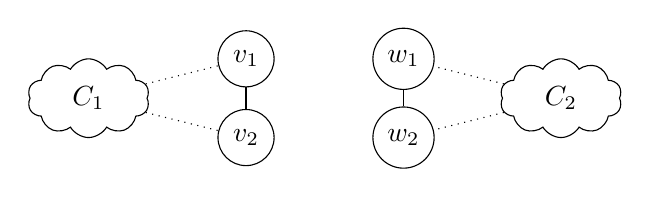
\begin{tikzpicture}
						\node[cloud, cloud puffs=10, cloud puff arc=120, aspect=2, minimum width=1.5cm, minimum height=1cm, draw] (c1)  at (-1,-0.5) {$C_1$};
						\node[circle, draw] (v1) at (1, 0) {$v_1$};
						\node[circle, draw] (v2) at (1, -1) {$v_2$};
						\draw[dotted] (c1) -- (v1);
						\draw[dotted] (c1) -- (v2);
						\draw (v1) -- (v2);
		
						\node[cloud, cloud puffs=10, cloud puff arc=120, aspect=2, minimum width=1.5cm, minimum height=1cm, draw] (c2)  at (5,-0.5) {$C_2$};
						\node[circle, draw] (w1) at (3, 0) {$w_1$};
						\node[circle, draw] (w2) at (3, -1) {$w_2$};
						\draw[dotted] (c2) -- (w1);
						\draw[dotted] (c2) -- (w2);
						\draw (w1) -- (w2);
					\end{tikzpicture}
				} $\Rightarrow$
				\resizebox {0.25\textwidth}{!}{
					\begin{tikzpicture}
						\node[cloud, cloud puffs=10, cloud puff arc=120, aspect=2, minimum width=1.5cm, minimum height=1cm, draw] (c1)  at (-1,-0.5) {$C_1$};
						\node[circle, draw] (v1) at (1, 0) {$v_1$};
						\node[circle, draw] (v2) at (1, -1) {$v_2$};
						\draw[dotted] (c1) -- (v1);
						\draw[dotted] (c1) -- (v2);
						\draw (v1) -- (w1);
		
						\node[cloud, cloud puffs=10, cloud puff arc=120, aspect=2, minimum width=1.5cm, minimum height=1cm, draw] (c2)  at (5,-0.5) {$C_2$};
						\node[circle, draw] (w1) at (3, 0) {$w_1$};
						\node[circle, draw] (w2) at (3, -1) {$w_2$};
						\draw[dotted] (c2) -- (w1);
						\draw[dotted] (c2) -- (w2);
						\draw (w1) -- (w2);
					\end{tikzpicture}
				} $\Rightarrow$
				\resizebox {0.25\textwidth}{!}{
					\begin{tikzpicture}
						\node[cloud, cloud puffs=10, cloud puff arc=120, aspect=2, minimum width=1.5cm, minimum height=1cm, draw] (c1)  at (-1,-0.5) {$C_1$};
						\node[circle, draw] (v1) at (1, 0) {$v_1$};
						\node[circle, draw] (v2) at (1, -1) {$v_2$};
						\draw[dotted] (c1) -- (v1);
						\draw[dotted] (c1) -- (v2);
						\draw (v1) -- (w1);
		
						\node[cloud, cloud puffs=10, cloud puff arc=120, aspect=2, minimum width=1.5cm, minimum height=1cm, draw] (c2)  at (5,-0.5) {$C_2$};
						\node[circle, draw] (w1) at (3, 0) {$w_1$};
						\node[circle, draw] (w2) at (3, -1) {$w_2$};
						\draw[dotted] (c2) -- (w1);
						\draw[dotted] (c2) -- (w2);
						\draw (v2) -- (w2);
					\end{tikzpicture}
				}
			\end{center}

			Let $C_1 = (V_1, E_1)$ and $C_2 = (V_2, E_2)$ be components of $G$. Furthermore, we consider $v_1, v_2 \in V_1$ to be adjacent vertices contained in a cycle of $C_1$ and $w_1, w_2 \in V_2$ to be adjacent vertices contained in a cycle of $C_2$. We always find those vertices since the graph's minimum degree exceeds or is equal to two (Lecture: \emph{Any graph $H$ with $\delta(H) \geq 2$ contains a cycle}).\\

			First, we remove the edges $\{v_1, v_2\} \in E_1$ and $\{w_1, w_2\} \in E_2$. Notably, neither $C_1$ nor $C_2$ have been disconnected since each of these edges is contained in a cycle and hence not crucial for the connectivity of $C_1$ and $C_2$. Now, we add the edges $\{v_1, w_1\}$ as well as $\{v_2, w_2\}$ and thereby connect $C_1$ with $C_2$.\\
			
			We can easily see that no degree has been changed. Each vertex has lost and gained one indicent edge. From these considerations, the graph's degree sequence has not been modified. Moreover, we have connected the two components without disconnecting one.

			Inductively, we are able to connect the entire graph and at the same time maintain it's degree sequence. Thus, a connected graph with the same degree sequence exists.

		\end{theorem}
	\end{solution}
	\newpage
	\begin{solution}{6}
		In the following I will proof that any tree with an even number of vertices has exactly one spanning subgraph in which every vertex has odd degree. 
		I will reduce the problem by recursively removing leaves until only the trivial case of two vertices is left. 
		First, I will proof the following lemma which then later is used to to proof the theorem. 
			
		\begin{lemma}{In a tree $T=(V,E)$ with $|V|>2$ if there is no vertex $u \in V$ connected to atleast two leaves $v_1, v_2 \in V$, there is a leaf $v \in V$ connected to a vertex $u$ with $deg(u) = 2$.}
			From the prerequisite that there is no vertex $u \in V$ connected to atleast two leaves, we know that all leaves are connected to different vertices. 
			Let's assume there is no such vertex $u$, then all vertices $u \in V$ connected two a leaf have to have $deg(u) \neq 2$. 
			Because $T$ is connected and $|V|>2$ all $u$ have to have an edge and cannot be a leaf itself, hence for all such $u$ $deg(u) \geq 3$. 
			By removing all leaves from $T$ we get $T'$ a subgraph of $T$. By removing the leaves only the degree of all $u$ connected to a leaf are reduced be one. 
			Then for all $u$ $deg(u) \geq 2$ in the subgraph $T'$. 
			Additionally, because the degree of all other vertices is not changed and they are no leaves the degree of all vertices of the resulting graph is greater or equal 2. 
			Thus using a lemma of the lecture the result graph has to have a cycle. 
			Because $T'$ is a subgraph of $T$ this is a contradiction to $T$ being acyclic. 
			Hence, there has to be a vertex $u$ connected to a leaf with $deg(u)=2$. 		
		\end{lemma}
					
		\begin{theorem}{Any tree with an even number of vertices has exactly one spanning subgraph in which every vertex has odd degree.}
			Let $T=(V, E)$ be a tree with even number. If $|V|=0$ or $|V|=2$ there is obviously exact one spanning subgraph. 
			In the following let $|V|>2$ and let $S$ be the set of edges of a spanning subgraph meeting the conditions stated above. \\
			In the lecture we proved that $T$ has atleast one leaf $v$. 
			Because any leaf only has one edge $(v,u)$, this edge has to be in $S$. 
			Additionally, if the edge $(v,u)$ is part of $S$ the condition that the degree of any vertex is odd is met for the leaf $v$. 
			Then always one of the following cases applies. 
			\begin{itemize}
				\item \textbf{Case 1:} There is one edge $u \in V$ connected to atleast two leaves $v_1, v_2 \in V$. \\
				We know that the edges $(u,v_1)$ and $(u,v_2)$ have to be in $S$. 
				If we remove $v_1$ and $v_2$ from T we again receive a tree $T'$ with an even number of vertices. 
				Additionally, if there is exactly one spanning subgraph for $T'$ with only odd degrees then there is also exactly one for $T$ which additionally covers the vertices $v_1$ and $v_2$. 
				Hence, either $|V- \{v_1,v_2\}| \leq 2$ and we know that there is exact one spanning subgraph meeting the conditions, or we can again apply case 1 or case 2. 
				
				\begin{center}
				\resizebox {0.25\textwidth}{!}{
					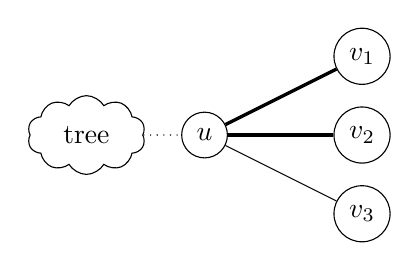
\begin{tikzpicture}
						\node[cloud, cloud puffs=10, cloud puff arc=120, aspect=2, minimum width=1.5cm, minimum height=1cm, draw] (c1)  at (-2.5,-0.5) {tree};
						\node[circle, draw] (u) at (-1, -0.5) {$u$};
						\node[circle, draw] (v1) at (1, 0.5) {$v_1$};
						\node[circle, draw] (v2) at (1, -0.5) {$v_2$};
						\node[circle, draw] (v3) at (1, -1.5) {$v_3$};
						\draw[very thick] (u) -- (v1);
						\draw[very thick] (u) -- (v2);
						\draw (u) -- (v3);
						\draw[dotted] (c1) -- (u);

					\end{tikzpicture}
				} $\Rightarrow$
				\resizebox {0.25\textwidth}{!}{
					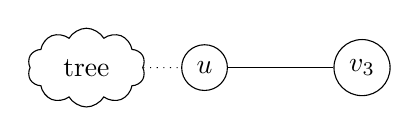
\begin{tikzpicture}
						\node[cloud, cloud puffs=10, cloud puff arc=120, aspect=2, minimum width=1.5cm, minimum height=1cm, draw] (c1)  at (-2.5,-0.5) {tree};
						\node[circle, draw] (u) at (-1, -0.5) {$u$};
						\node[circle, draw] (v3) at (1, -0.5) {$v_3$};
						\draw (u) -- (v3);
						\draw[dotted] (c1) -- (u);
					\end{tikzpicture}
				}
			\end{center}
			
				
				\item \textbf{Case 2:} There is no edge $u \in V$ connected to atleast two leaves $v_1, v_2 \in V$. \\
				Using the lemma we can find a leaf $v \in V$ with an edge $(v,u) \in E$ with $deg(v)=2$. 
				We know that the edge $(v,u)$ has to be in $S$. 
				Additionally, we know that the degree of $u$ in any spanning subgraph meeting the conditions has to be odd, so the second edge $(u,t)$ with $t \in V$ cannot be in $S$. 
				If we remove $u$ and $v$ from T we again receive a tree with an even number of vertices. 
				Hence, either $|V- \{v,u\}| \leq 2$ and we know that there is exact one spanning subgraph meeting the conditions, or we can again apply case 1 or case 2. 
				\begin{center}
				\resizebox {0.25\textwidth}{!}{
					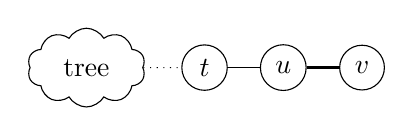
\begin{tikzpicture}
						\node[cloud, cloud puffs=10, cloud puff arc=120, aspect=2, minimum width=1.5cm, minimum height=1cm, draw] (c1)  at (-2.5,-0.5) {tree};
						\node[circle, draw] (t) at (-1, -0.5) {$t$};
						\node[circle, draw] (u) at (0, -0.5) {$u$};
						\node[circle, draw] (v) at (1, -0.5) {$v$};
						\draw[dotted] (c1) -- (t);
						\draw (t) -- (u);			
						\draw[very thick] (u) -- (v);

					\end{tikzpicture}
				} $\Rightarrow$
				\resizebox {0.25\textwidth}{!}{
					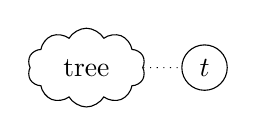
\begin{tikzpicture}
						\node[cloud, cloud puffs=10, cloud puff arc=120, aspect=2, minimum width=1.5cm, minimum height=1cm, draw] (c1)  at (-2.5,-0.5) {tree};
						\node[circle, draw] (t) at (-1, -0.5) {$t$};
						\draw[dotted] (c1) -- (t);
					\end{tikzpicture}
				}
			\end{center}
			
			
			\end{itemize}
		
		All in all we can always find edges in $T$ which have to be part of $S$ and thus reducing $T$ until there is only the trivial solution. 
		Thus the theorem is proven by induction. 
		\end{theorem}
	\end{solution} 
	\newpage
	\begin{solution}{7}
		For a set $C = \{G_1, ..., G_n\}$ of connected components:\\
		\begin{align}
			\pi(C)&= \sum_{i = 1}^n \frac{|\{v \in V(G_i)\ |\ d(v) \text{ odd}\}|}{2}&
		\end{align}
	\end{solution} 
	\newpage
	\begin{solution}{8}
		
	\end{solution}
	
\end{document}